\raggedbottom

\section{Ejercicio 1: Interrupciones con botones de baja y alta prioridad
}
Para este programa se usará el código del TP1 como base, el cual se modificará para hacer interrupciones al led del TP1 con botones de baja y alta prioridad.
Para conseguir esto se agregaron las siguientes definiciones en el archivo main.c:

\begin{itemize}
    \item Se definió la dirección base \textbf{AFIO\_BASE} con la dirección del registro AFIO.
    \item Se definió la dirección base \textbf{EXTI\_BASE} con la dirección del registro EXTI, el cual se utiliza para configurar las interrupciones externas.
    \item Se definió la dirección base \textbf{NVIC\_BASE} con la dirección del registro NVIC, el cual se utiliza para configurar las interrupciones en el NVIC.
    \item Se definió el registro \textbf{AFIO\_EXTICR1} con la dirección del registro AFIO\_EXTICR1, el cual se utiliza para configurar el pin del botón como fuente de interrupción externa.
    \item Se definió el registro \textbf{EXTI\_IMR} con la dirección del registro EXTI\_IMR, el cual se utiliza para habilitar las interrupciones de los pines configurados.
    \item Se definió el registro \textbf{EXTI\_FTSR} con la dirección del registro EXTI\_FTSR, el cual se utiliza para configurar la interrupción por flanco de bajada.
    \item Se definió el registro \textbf{EXTI\_PR} con la dirección del registro EXTI\_PR, el cual se utiliza para limpiar las banderas de interrupción.
    \item Se definió el registro \textbf{NVIC\_ISER0} con la dirección del registro NVIC\_ISER0, el cual se utiliza para habilitar las interrupciones en el NVIC.
    \item Se definió el registro \textbf{NVIC\_IPR1} con la dirección del registro NVIC\_IPR1, el cual se utiliza para configurar la prioridad de las interrupciones de los IRQ 4 a 7.
    \item Se definió el registro \textbf{NVIC\_IPR2} con la dirección del registro NVIC\_IPR2, el cual se utiliza para configurar la prioridad de las interrupciones de los IRQ 8 a 11.
    \item Se definieron las mascaras \textbf{GPIOA4} , \textbf{GPIOA5} y \textbf{GPIOA6}
\end{itemize}


\begin{figure}[H]
    \centering
    
\includegraphics[width=0.5\textwidth]{images/definiciones.png}
    \caption*{Definiciones de los registros en main.c}
    \label{fig:led}
\end{figure}

A continuación agregamos las funciones de interrupción para los botones, las cuales se encargan de encender y apagar el led correspondiente al botón presionado. Para el botón de baja prioridad (A1) se encenderá el led del pin A6, y para el botón de alta prioridad (A2) se encenderá el led del pin A5.

\begin{figure}[H]
    \centering
    
\includegraphics[width=0.5\textwidth]{images/funciones.png}
    \caption*{Agregado de funciones para interrupciones}
    \label{fig:funciones}
\end{figure}


Ahora pasamos a modificar la función \textbf{main}

\begin{figure}[H]
    \centering
    
\includegraphics[width=0.5\textwidth]{images/main.png}
    \caption*{Configuración de los pines y las interrupciones en main}
    \label{fig:main}
\end{figure}

Primero habilitamos los clocks del GPIO y AFIO, luego configuramos los pines A4, A5 y A6 como salida, y los A1 y A2 como entrada con pull-up. Luego asociamos el pin GPIO a la línea EXTI y pasamos a configurar las interrupciones como flancos descendentes, por ultimo configuramos el NVIC con las prioridades correspondientes.


\begin{figure}[H]
    \centering
    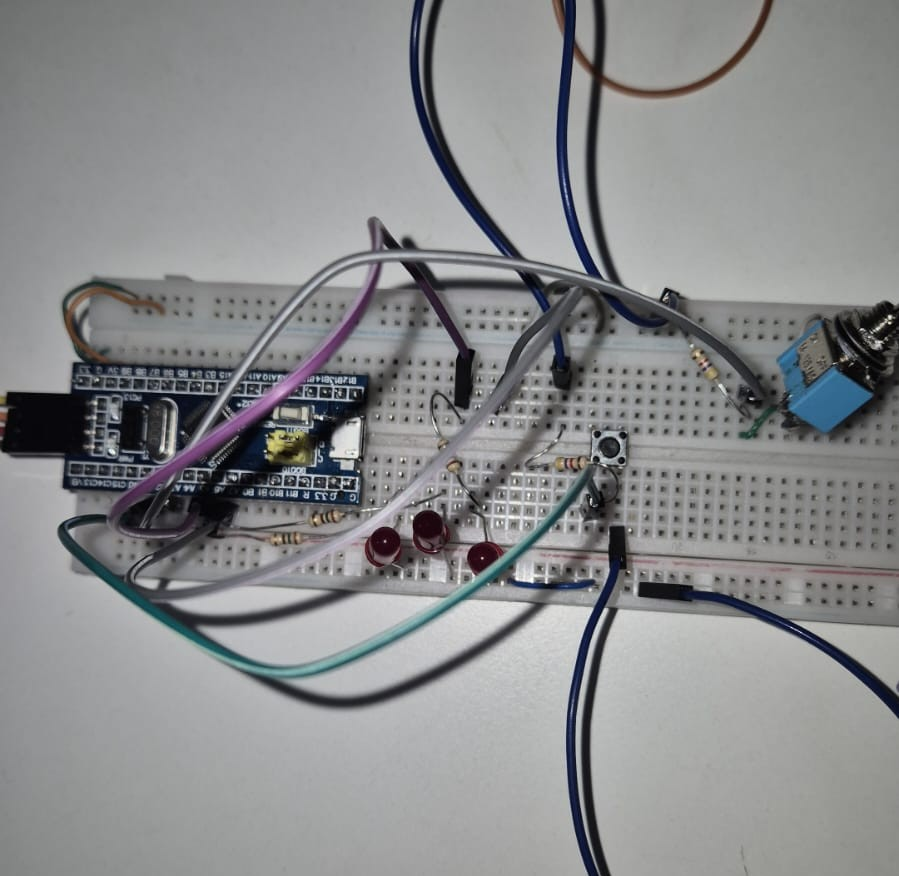
\includegraphics[width=0.45\textwidth]{images/proto1.jpeg}
    \caption*{Resultado final del ejercicio 1}
    \label{fig:resultado}
\end{figure}

El funcionamiento es el siguiente: Al iniciar el led del pin A4 se mantiene en un loop constante de encender y apagar, si se interrumple mediante el botón de baja prioridad (A1) el led del pin A6 se enciende y el del pin A4 se apaga, si se interrumpe mediante el botón de alta prioridad (A2) el led del pin A5 se enciende y el del pin A4 se apaga. Si mediante la interrupcion de baja prioridad se interrumpe con alta prioridad, el led del pin A5 se enciende y el del pin A6 se apaga, hasta terminar su ciclo de 5 encendidos y apagados, y luego el led A6 termina su ciclo donde lo dejo para luego volver al loop principal. 

